%% bare_conf.tex
%% V1.4b
%% 2015/08/26
%% by Michael Shell
%% See:
%% http://www.michaelshell.org/
%% for current contact information.
%%
%% This is a skeleton file demonstrating the use of IEEEtran.cls
%% (requires IEEEtran.cls version 1.8b or later) with an IEEE
%% conference paper.
%%
%% Support sites:
%% http://www.michaelshell.org/tex/ieeetran/
%% http://www.ctan.org/pkg/ieeetran
%% and
%% http://www.ieee.org/

%%*************************************************************************
%% Legal Notice:
%% This code is offered as-is without any warranty either expressed or
%% implied; without even the implied warranty of MERCHANTABILITY or
%% FITNESS FOR A PARTICULAR PURPOSE!
%% User assumes all risk.
%% In no event shall the IEEE or any contributor to this code be liable for
%% any damages or losses, including, but not limited to, incidental,
%% consequential, or any other damages, resulting from the use or misuse
%% of any information contained here.
%%
%% All comments are the opinions of their respective authors and are not
%% necessarily endorsed by the IEEE.
%%
%% This work is distributed under the LaTeX Project Public License (LPPL)
%% ( http://www.latex-project.org/ ) version 1.3, and may be freely used,
%% distributed and modified. A copy of the LPPL, version 1.3, is included
%% in the base LaTeX documentation of all distributions of LaTeX released
%% 2003/12/01 or later.
%% Retain all contribution notices and credits.
%% ** Modified files should be clearly indicated as such, including  **
%% ** renaming them and changing author support contact information. **
%%*************************************************************************


% *** Authors should verify (and, if needed, correct) their LaTeX system  ***
% *** with the testflow diagnostic prior to trusting their LaTeX platform ***
% *** with production work. The IEEE's font choices and paper sizes can   ***
% *** trigger bugs that do not appear when using other class files.       ***                          ***
% The testflow support page is at:
% http://www.michaelshell.org/tex/testflow/



\documentclass[conference]{IEEEtran}
% Some Computer Society conferences also require the compsoc mode option,
% but others use the standard conference format.
%
% If IEEEtran.cls has not been installed into the LaTeX system files,
% manually specify the path to it like:
% \documentclass[conference]{../sty/IEEEtran}


% Some very useful LaTeX packages include:
% (uncomment the ones you want to load)


% *** MISC UTILITY PACKAGES ***
%
%\usepackage{ifpdf}
% Heiko Oberdiek's ifpdf.sty is very useful if you need conditional
% compilation based on whether the output is pdf or dvi.
% usage:
% \ifpdf
%   % pdf code
% \else
%   % dvi code
% \fi
% The latest version of ifpdf.sty can be obtained from:
% http://www.ctan.org/pkg/ifpdf
% Also, note that IEEEtran.cls V1.7 and later provides a builtin
% \ifCLASSINFOpdf conditional that works the same way.
% When switching from latex to pdflatex and vice-versa, the compiler may
% have to be run twice to clear warning/error messages.






% *** CITATION PACKAGES ***
%
%\usepackage{cite}
% cite.sty was written by Donald Arseneau
% V1.6 and later of IEEEtran pre-defines the format of the cite.sty package
% \cite{} output to follow that of the IEEE. Loading the cite package will
% result in citation numbers being automatically sorted and properly
% "compressed/ranged". e.g., [1], [9], [2], [7], [5], [6] without using
% cite.sty will become [1], [2], [5]--[7], [9] using cite.sty. cite.sty's
% \cite will automatically add leading space, if needed. Use cite.sty's
% noadjust option (cite.sty V3.8 and later) if you want to turn this off
% such as if a citation ever needs to be enclosed in parenthesis.
% cite.sty is already installed on most LaTeX systems. Be sure and use
% version 5.0 (2009-03-20) and later if using hyperref.sty.
% The latest version can be obtained at:
% http://www.ctan.org/pkg/cite
% The documentation is contained in the cite.sty file itself.






% *** GRAPHICS RELATED PACKAGES ***
%
\ifCLASSINFOpdf
  % \usepackage[pdftex]{graphicx}
  % declare the path(s) where your graphic files are
  % \graphicspath{{../pdf/}{../jpeg/}}
  % and their extensions so you won't have to specify these with
  % every instance of \includegraphics
  % \DeclareGraphicsExtensions{.pdf,.jpeg,.png}
\else
  % or other class option (dvipsone, dvipdf, if not using dvips). graphicx
  % will default to the driver specified in the system graphics.cfg if no
  % driver is specified.
  % \usepackage[dvips]{graphicx}
  % declare the path(s) where your graphic files are
  % \graphicspath{{../eps/}}
  % and their extensions so you won't have to specify these with
  % every instance of \includegraphics
  % \DeclareGraphicsExtensions{.eps}
\fi
% graphicx was written by David Carlisle and Sebastian Rahtz. It is
% required if you want graphics, photos, etc. graphicx.sty is already
% installed on most LaTeX systems. The latest version and documentation
% can be obtained at:
% http://www.ctan.org/pkg/graphicx
% Another good source of documentation is "Using Imported Graphics in
% LaTeX2e" by Keith Reckdahl which can be found at:
% http://www.ctan.org/pkg/epslatex
%
% latex, and pdflatex in dvi mode, support graphics in encapsulated
% postscript (.eps) format. pdflatex in pdf mode supports graphics
% in .pdf, .jpeg, .png and .mps (metapost) formats. Users should ensure
% that all non-photo figures use a vector format (.eps, .pdf, .mps) and
% not a bitmapped formats (.jpeg, .png). The IEEE frowns on bitmapped formats
% which can result in "jaggedy"/blurry rendering of lines and letters as
% well as large increases in file sizes.
%
% You can find documentation about the pdfTeX application at:
% http://www.tug.org/applications/pdftex





% *** MATH PACKAGES ***
%
%\usepackage{amsmath}
% A popular package from the American Mathematical Society that provides
% many useful and powerful commands for dealing with mathematics.
%
% Note that the amsmath package sets \interdisplaylinepenalty to 10000
% thus preventing page breaks from occurring within multiline equations. Use:
%\interdisplaylinepenalty=2500
% after loading amsmath to restore such page breaks as IEEEtran.cls normally
% does. amsmath.sty is already installed on most LaTeX systems. The latest
% version and documentation can be obtained at:
% http://www.ctan.org/pkg/amsmath





% *** SPECIALIZED LIST PACKAGES ***
%
%\usepackage{algorithmic}
% algorithmic.sty was written by Peter Williams and Rogerio Brito.
% This package provides an algorithmic environment fo describing algorithms.
% You can use the algorithmic environment in-text or within a figure
% environment to provide for a floating algorithm. Do NOT use the algorithm
% floating environment provided by algorithm.sty (by the same authors) or
% algorithm2e.sty (by Christophe Fiorio) as the IEEE does not use dedicated
% algorithm float types and packages that provide these will not provide
% correct IEEE style captions. The latest version and documentation of
% algorithmic.sty can be obtained at:
% http://www.ctan.org/pkg/algorithms
% Also of interest may be the (relatively newer and more customizable)
% algorithmicx.sty package by Szasz Janos:
% http://www.ctan.org/pkg/algorithmicx




% *** ALIGNMENT PACKAGES ***
%
%\usepackage{array}
% Frank Mittelbach's and David Carlisle's array.sty patches and improves
% the standard LaTeX2e array and tabular environments to provide better
% appearance and additional user controls. As the default LaTeX2e table
% generation code is lacking to the point of almost being broken with
% respect to the quality of the end results, all users are strongly
% advised to use an enhanced (at the very least that provided by array.sty)
% set of table tools. array.sty is already installed on most systems. The
% latest version and documentation can be obtained at:
% http://www.ctan.org/pkg/array


% IEEEtran contains the IEEEeqnarray family of commands that can be used to
% generate multiline equations as well as matrices, tables, etc., of high
% quality.




% *** SUBFIGURE PACKAGES ***
%\ifCLASSOPTIONcompsoc
%  \usepackage[caption=false,font=normalsize,labelfont=sf,textfont=sf]{subfig}
%\else
%  \usepackage[caption=false,font=footnotesize]{subfig}
%\fi
% subfig.sty, written by Steven Douglas Cochran, is the modern replacement
% for subfigure.sty, the latter of which is no longer maintained and is
% incompatible with some LaTeX packages including fixltx2e. However,
% subfig.sty requires and automatically loads Axel Sommerfeldt's caption.sty
% which will override IEEEtran.cls' handling of captions and this will result
% in non-IEEE style figure/table captions. To prevent this problem, be sure
% and invoke subfig.sty's "caption=false" package option (available since
% subfig.sty version 1.3, 2005/06/28) as this is will preserve IEEEtran.cls
% handling of captions.
% Note that the Computer Society format requires a larger sans serif font
% than the serif footnote size font used in traditional IEEE formatting
% and thus the need to invoke different subfig.sty package options depending
% on whether compsoc mode has been enabled.
%
% The latest version and documentation of subfig.sty can be obtained at:
% http://www.ctan.org/pkg/subfig




% *** FLOAT PACKAGES ***
%
%\usepackage{fixltx2e}
% fixltx2e, the successor to the earlier fix2col.sty, was written by
% Frank Mittelbach and David Carlisle. This package corrects a few problems
% in the LaTeX2e kernel, the most notable of which is that in current
% LaTeX2e releases, the ordering of single and double column floats is not
% guaranteed to be preserved. Thus, an unpatched LaTeX2e can allow a
% single column figure to be placed prior to an earlier double column
% figure.
% Be aware that LaTeX2e kernels dated 2015 and later have fixltx2e.sty's
% corrections already built into the system in which case a warning will
% be issued if an attempt is made to load fixltx2e.sty as it is no longer
% needed.
% The latest version and documentation can be found at:
% http://www.ctan.org/pkg/fixltx2e


\usepackage{stfloats}
% stfloats.sty was written by Sigitas Tolusis. This package gives LaTeX2e
% the ability to do double column floats at the bottom of the page as well
% as the top. (e.g., "\begin{figure*}[!b]" is not normally possible in
% LaTeX2e). It also provides a command:
%\fnbelowfloat
% to enable the placement of footnotes below bottom floats (the standard
% LaTeX2e kernel puts them above bottom floats). This is an invasive package
% which rewrites many portions of the LaTeX2e float routines. It may not work
% with other packages that modify the LaTeX2e float routines. The latest
% version and documentation can be obtained at:
% http://www.ctan.org/pkg/stfloats
% Do not use the stfloats baselinefloat ability as the IEEE does not allow
% \baselineskip to stretch. Authors submitting work to the IEEE should note
% that the IEEE rarely uses double column equations and that authors should try
% to avoid such use. Do not be tempted to use the cuted.sty or midfloat.sty
% packages (also by Sigitas Tolusis) as the IEEE does not format its papers in
% such ways.
% Do not attempt to use stfloats with fixltx2e as they are incompatible.
% Instead, use Morten Hogholm'a dblfloatfix which combines the features
% of both fixltx2e and stfloats:
%
% \usepackage{dblfloatfix}
% The latest version can be found at:
% http://www.ctan.org/pkg/dblfloatfix



% *** PDF, URL AND HYPERLINK PACKAGES ***
%
%\usepackage{url}
% url.sty was written by Donald Arseneau. It provides better support for
% handling and breaking URLs. url.sty is already installed on most LaTeX
% systems. The latest version and documentation can be obtained at:
% http://www.ctan.org/pkg/url
% Basically, \url{my_url_here}.




% *** Do not adjust lengths that control margins, column widths, etc. ***
% *** Do not use packages that alter fonts (such as pslatex).         ***
% There should be no need to do such things with IEEEtran.cls V1.6 and later.
% (Unless specifically asked to do so by the journal or conference you plan
% to submit to, of course. )


% correct bad hyphenation here
\hyphenation{op-tical net-works semi-conduc-tor}

\usepackage[]{graphicx} % added to make your file compilable
\usepackage{subfigure}
\usepackage{fixltx2e}
\usepackage{refstyle}
\usepackage{float}
\usepackage{multicol}
\usepackage{multirow}
\usepackage{booktabs}
\usepackage{diagbox}
\usepackage{tabularx}
\usepackage{fancyhdr}
\usepackage{fancyhdr}
\usepackage{amsmath}

\def\RSfigtxt{Fig.\,}%
\def\RSfigstxt{Figs~}%
\def\RSFigtxt{Fig.\,}%
\def\RSFigstxt{Figs~}%



\begin{document}
%
% paper title
% Titles are generally capitalized except for words such as a, an, and, as,
% at, but, by, for, in, nor, of, on, or, the, to and up, which are usually
% not capitalized unless they are the first or last word of the title.
% Linebreaks \\ can be used within to get better formatting as desired.
% Do not put math or special symbols in the title.

\title{Multi-parameter regression control of snake-like robots based on learning experience}

% author names and affiliations
% use a multiple column layout for up to three different
% affiliations
%\author{\IEEEauthorblockN{Shanshan Xiao}
%\IEEEauthorblockA{School of Data and Computer Science\\
%Sun yat-sen University\\
%Guangzhou, China\\
%Email: camembert33@icloud.com}
%\and
%\IEEEauthorblockN{Zhenshan Bing}
%\IEEEauthorblockA{Department of Computer Science\\
%Technical University of Munich\\
%Munich, Germany\\
%Email: bing@in.tum.de}
%\and
%\IEEEauthorblockN{Kai Huang}
%\IEEEauthorblockA{School of Data and Computer Science\\
%Sun yat-sen University\\
%Guangzhou, China\\
%Email: huangk36@mail.sysu.edu.cn}
%\and
%\IEEEauthorblockN{Yuhong Huang}
%\IEEEauthorblockA{School of Data and Computer Science\\
%Sun yat-sen University\\
%Guangzhou, China\\
%Email: huangyh43@qq.com}}

% conference papers do not typically use \thanks and this command
% is locked out in conference mode. If really needed, such as for
% the acknowledgment of grants, issue a \IEEEoverridecommandlockouts
% after \documentclass

% for over three affiliations, or if they all won't fit within the width
% of the page, use this alternative format:
%
\author{\IEEEauthorblockN{
	Zhiyong Jian\IEEEauthorrefmark{1}	
	Yuhong Huang\IEEEauthorrefmark{2},
	Linlin Liu\IEEEauthorrefmark{1},
	Long Cheng{3}\IEEEauthorrefmark{3} and
	Kai Huang\IEEEauthorrefmark{1}
}
\IEEEauthorblockA{\IEEEauthorrefmark{1}School of Data and Computer Science,Sun yat-sen University, Guangzhou, China, Email: jianzhy5@mail2.sysu.edu.cn}
\IEEEauthorblockA{\IEEEauthorrefmark{2}College of Computer, National University of Defense Technology, ChangSha, China, Email: huangyuhong17@nudt.edu.cn}
\IEEEauthorblockA{\IEEEauthorrefmark{1}Email: liull28@mail2.sysu.edu.cn}
\IEEEauthorblockA{\IEEEauthorrefmark{3}Email: chengl@in.tum.de}
\IEEEauthorblockA{\IEEEauthorrefmark{1}Email: huangk36@mail.sysu.edu.cn}}




% use for special paper notices
%\IEEEspecialpapernotice{(Invited Paper)}




% make the title area
\maketitle
\thispagestyle{fancy}	
\cfoot{\thepage}
\pagestyle{fancy}
\cfoot{\thepage}
% As a general rule, do not put math, special symbols or citations
% in the abstract
\begin{abstract}\,
Snake-like robots have a very good application prospect in complex environments because of their high complexity and multi-joint feature. It is difficult to manipulate the robot movement in real time. Thus, the autonomous mobility of snake-like robots is one of the main research directions. A new control framework based on machine learning is presented on this paper. Through the clustering algorithm, training data is classified into several clusters. The motion control of snake-like robots involves multiple regression problems because of multi-parameter motion control strategy. We propose a new strategy based on the data from previous training and transform the multiple regression into a unit regression problem to modify the parameter. We have experimentally verified that the robots are adaptable for different pipeline environment based on our algorithm framework.
\end{abstract}


\renewcommand\IEEEkeywordsname{Keywords}
\begin{IEEEkeywords}
Snake-like robot; autonomous ability; pipe climbing; multiple regression
\end{IEEEkeywords}

% For peer review papers, you can put extra information on the cover
% page as needed:
% \ifCLASSOPTIONpeerreview
% \begin{center} \bfseries EDICS Category: 3-BBND \end{center}
% \fi
%
% For peerreview papers, this IEEEtran command inserts a page break and
% creates the second title. It will be ignored for other modes.
\IEEEpeerreviewmaketitle

\section{Introduction}
% no \IEEEPARstart
Snake-like robots, with multiple joints and degree of freedom, have strong mobility in complex and unknown terrains\cite{Chirikjian1995The}. Snake-like robots adapt themselves to multiple robotic mobility occasions such as disaster rescuing\cite{DogAndSnake}, factory pipe maintenance\cite{ACMTutorial} and scientific exploration\cite{Kuwada2007Snake}. The early version of snake-like robots used parallel connection structure to connect each two modules, only achieving a plane movement\cite{mori2002three}. Later, with the advent of orthogonal and universal joint structure\cite{1014757}\cite{Date2005Control}\cite{GaitBasedCompliant}, snake-like robots can be applied to three-dimensional space movement, which strengthens snake-like robots' mobility in varied topography. Over the years, more and more gaits that can traverse a variety of terrains, including flat ground and pipes have been developed\cite{5152862}\cite{5602354}. However, it is challenging to make robots move in complex environment without real-time human intervention such as parameters adjustment.

It's necessary for the robots to have autonomous mobility if we want them to move in complex or unknown environment such as climbing the outdoor pipeline for maintenance. Actually, by setting the accurate parameters of motion, snake-like robots can travel along the pipes with different diameters by rolling gait. However, the motions of snake-like robots are not efficient under the real-time control of human. Our goal is to develop a new autonomous control strategy for the motion of snake-like robots. We propose a new control strategy based on learning experience of robots . The robots' adaptive motion can improve adaptability in different movement environments.

This paper applies the new control strategy to the our existing snake-like robot platform, which is shown in \figref{fig:snake_like_robot_a}. The rotation axis of the adjacent joints of our robot are orthogonal and the rotation axis of robot's joints are perpendicular to the its body. We construct the simulation model \figref{fig:snake_like_robot_b} and embed a set of sensors such as accelerometer and gyro to realize the robot feedback control.
\begin{figure}[H]
	\centering
	\subfigure[Reality robot]{
		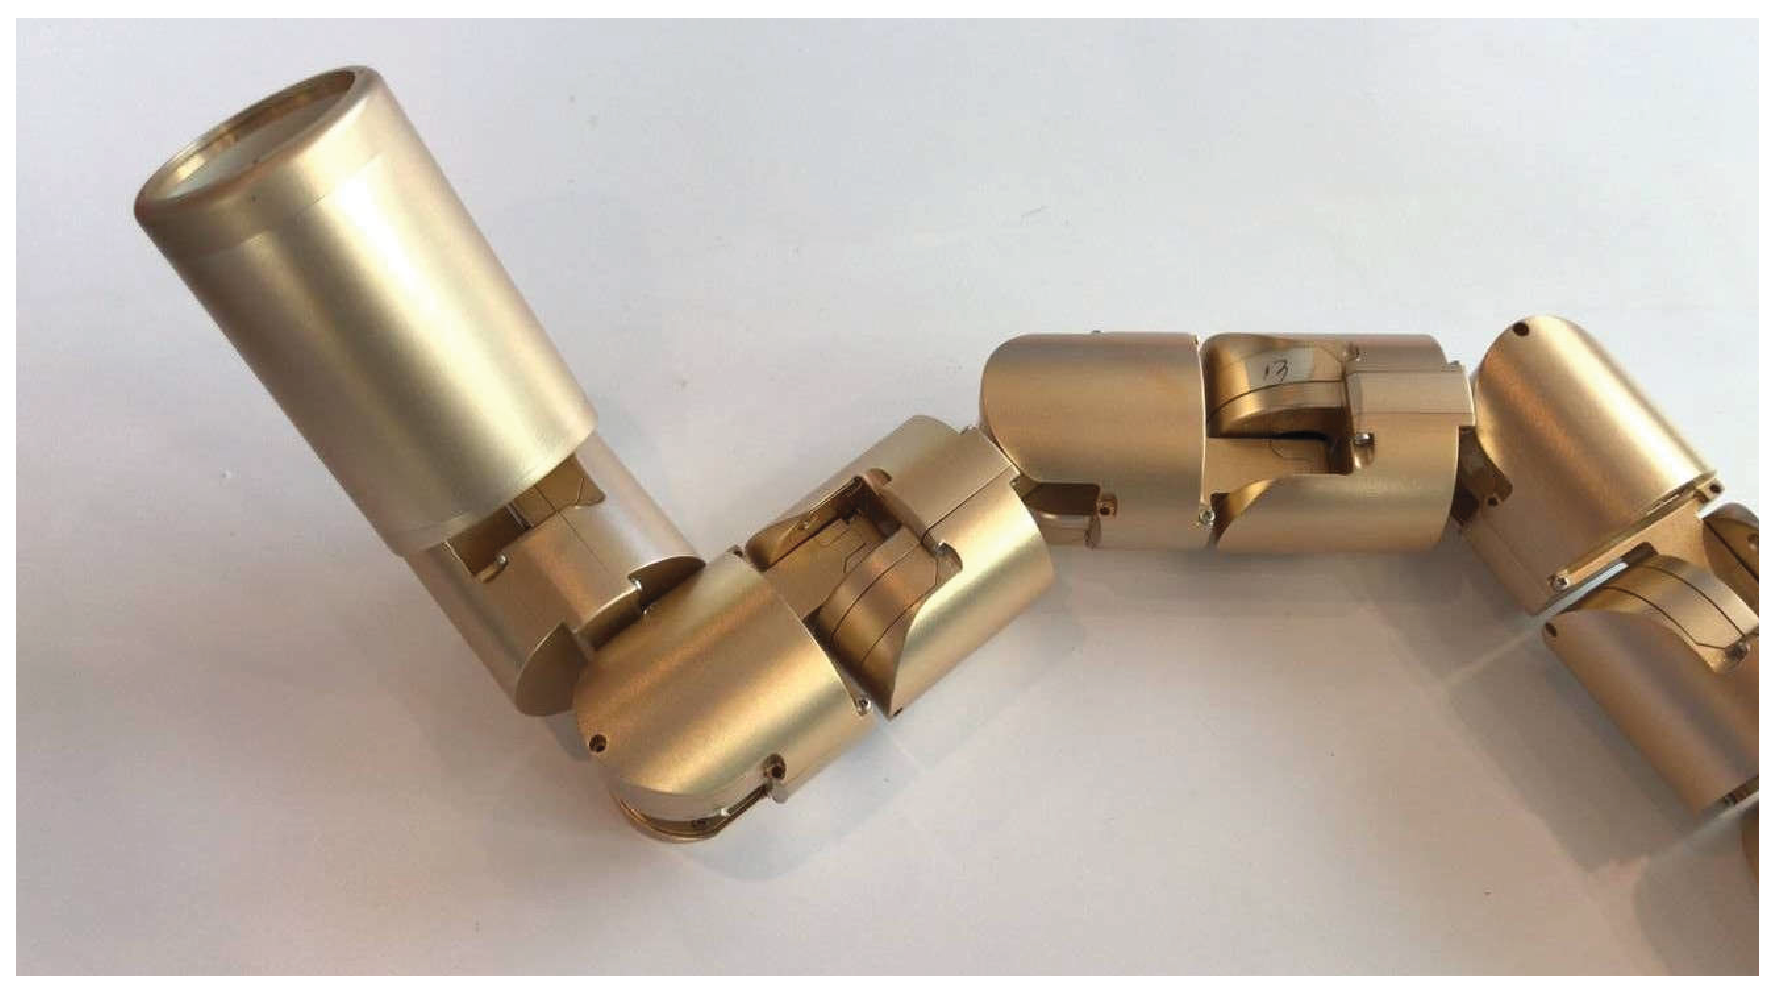
\includegraphics[width=1.5in,height=0.75in]{fig/relative/realSnake}
		\figlabel{fig:snake_like_robot_a}
	}
	\subfigure[Simulation robot]{
		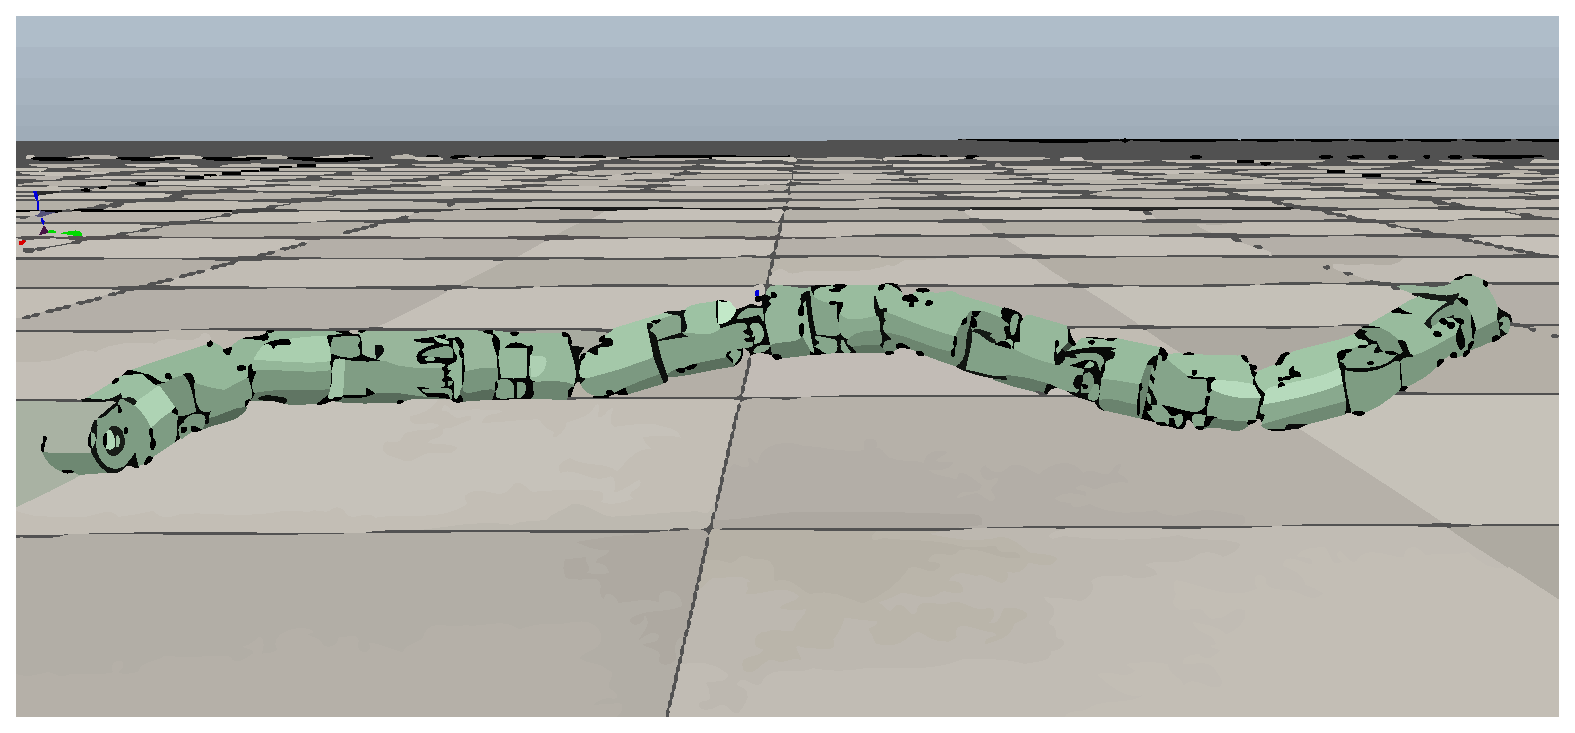
\includegraphics[width=1.5in,height=0.75in]{fig/relative/simulateSnake}
		\figlabel{fig:snake_like_robot_b}
	}
	\caption{The Snake-like robot}
	\figlabel{fig:snake_like_robot}
\end{figure}

The whole process of our control strategy is divided into two parts:

\begin{enumerate}
	\item data acquisition and preprocessing,
	\item real-time data feedback and multi-parameter regression control.
\end{enumerate}

The simulation environment is the pipe climbing, which can be used in cable detection of cable-stayed bridge. In the first part, we collect data in pipes with different diameter as training set. To reduce time of calculation in feed-back control, we adopt clustering algorithm\cite{Cluseter_ICT}\cite{KmeansAndDeepLearning}. In the second part, we apply regression and feed-back control based on previous training data on the motion of robots. We utilize the entropy variance\cite{WaveformEntropyVariance}\cite{EntropyandVarianceasRiskMeasure}\cite{UsingEntropyAndVariance} to measure the effect of the control parameters on the motion and select the most sensitive parameter which has the greatest effect on motion. By transforming the multiple regression into the unit regression and combining the weighted least squares algorithm\cite{gradientMethod}\cite{MSEestimates}, we finally get a fitted regression function and modify the most sensitive parameter.

The contribution of this paper are:

\begin{itemize}
	\item A new framework for robot adaptive control is proposed.
 	This framework greatly reduces the amount of  effort of the regression calculation because of the use of clustering algorithm for data preprocessing as well as the classification of real-time data.
	\item A solution to the problem of multiple regression is proposed.
	Multi-parameter regression is seen as a multiple regression problem. The entropy variance is utilized to select the parameters which are the most sensitive currently, and the rest of the parameters are hysteresis. Therefore, by regressing the sensitive parameter instead of all the parameters, the multiple regression is transformed into the unit regression problem.
\end{itemize}




\section{Relative work}
Currently, a widely used of control strategy for snake-like robots is based on the sinusoidal motion model\cite{HiroseSine} which is proposed by professor Hirose. After that, Tesch et al. proposed a parametric equation based on the sinusoidal model for a snake-shaped robot with three-dimensional athleticism\cite{ChosetSine}. This parametric equation simplifies the control strategy of the snake-like robots and allows the robot to determine the movement model of the machine with a small amount of control parameters.

The sinusoidal motion model function is shown in the following formula:
\begin{eqnarray}\label{basicRoll}
T_i=\left\{
\begin{array}{lr}
A\cdot \sin (\omega \cdot t + i\cdot \varepsilon )&odd\\
A\cdot \sin (\omega \cdot t + i\cdot \varepsilon +  \frac{\pi}{2})&even
\end{array}
\right.
\end{eqnarray}

By modifying the amplitude $A$, phase $\varepsilon$, and angular rate $\omega$ in Eq.\ref{basicRoll}, the maximum rotation angle of joints, the robot shape period and the motion rate of the serpentine robot are changed. In order to ensure that snake-like robots can be applied to a wider scene, robots need to have autonomous adaptability to the environment.

%To make the robots adapt to the unknown environment, the method which use the sensors to perceive the environment and embed the environment perception rules, has been widely used\cite{CPGenabling}\cite{GaitBasedCompliant}\cite{BalancingAndControl}\cite{FeedbackControlOfSoft}. Tang et al. proposed a control strategy based on CPG(central pattern generator) model\cite{CPGenabling}. Rollinson et al. proposed a snake-like robot adaptive control based on state estimation\cite{GaitBasedCompliant}. However, a complete correlation prediction model of control parameters is not given in their paper. As their methods is a gradient model based on state estimation, thus they are not suited to the mutation environment. What's more, there are researchers that have proposed a neural network model combined with physical environment information to determine the control scheme\cite{InformationDriven}\cite{NovelPlasticityRule}\cite{MissileSystems}\cite{NeuroFuzzyBayesian}. This model is only the control suggestion and may not make a good effect on motion in real-time motion of the robot. 
To make the robots adapt to the unknown environment, the method which use the sensors to perceive the environment and embed the environment perception rules, has been widely used\cite{CPGenabling}\cite{GaitBasedCompliant}\cite{BalancingAndControl}\cite{FeedbackControlOfSoft}. Tang et al. proposed a control strategy based on CPG(central pattern generator) model\cite{CPGenabling}. Rollinson et al. proposed a snake-like robot adaptive control based on state estimation\cite{GaitBasedCompliant}. However, a complete correlation prediction model of control parameters is not given in their paper. As their methods is a gradient model based on state estimation, they are not suited to the mutation environment.
%To adapt to the environment, the method which use the sensors to perceive the environment and embed the environment perception rules, has been widely used\cite{CPGenabling}\cite{GaitBasedCompliant}\cite{BalancingAndControl}\cite{FeedbackControlOfSoft}. Tang et al. proposed a control strategy based on CPG(central pattern generator) model\cite{CPGenabling}. They achieve to control the gait change to adapt to the environment by taking speed as a measure,  embedding several gaits to the robots and combining with CPG control according to the environment. Rollinson et al. proposed a snake-like robot adaptive control based on state estimation\cite{GaitBasedCompliant}. A complete correlation prediction model of control parameters is not given in their paper. As it is based on state estimation, this method is a step-by-step change model, thus it is not suited to the mutation environment. %There are some algorithms of machine learning in the robot control applications\cite{InformationDriven}\cite{NovelPlasticityRule}\cite{MissileSystems}\cite{NeuroFuzzyBayesian}. They only give control program conversion but do not provide changes in the control strategy.

On the application of machine learning in the field of robot control, there are researchers that have proposed a neural network model combined with physical environment information to determine the control scheme\cite{InformationDriven}\cite{NovelPlasticityRule}\cite{MissileSystems}\cite{NeuroFuzzyBayesian}. This model is only the control suggestion and may not make a good effect on motion in real-time motion of the robot. 

In this paper, a control strategy by experience-based learning  is proposed. Combined with the clustering\cite{Cluseter_ICT}\cite{KmeansAndDeepLearning} and the multi-parameter regression, we realize the real-time autonomous change of multiple control parameters in the robots' movement.

\section{Adaptive control strategy}

The intelligent control strategy proposed in this paper is shown in \figref{fig:stepMap}.
\begin{figure}[H]
	\centering
	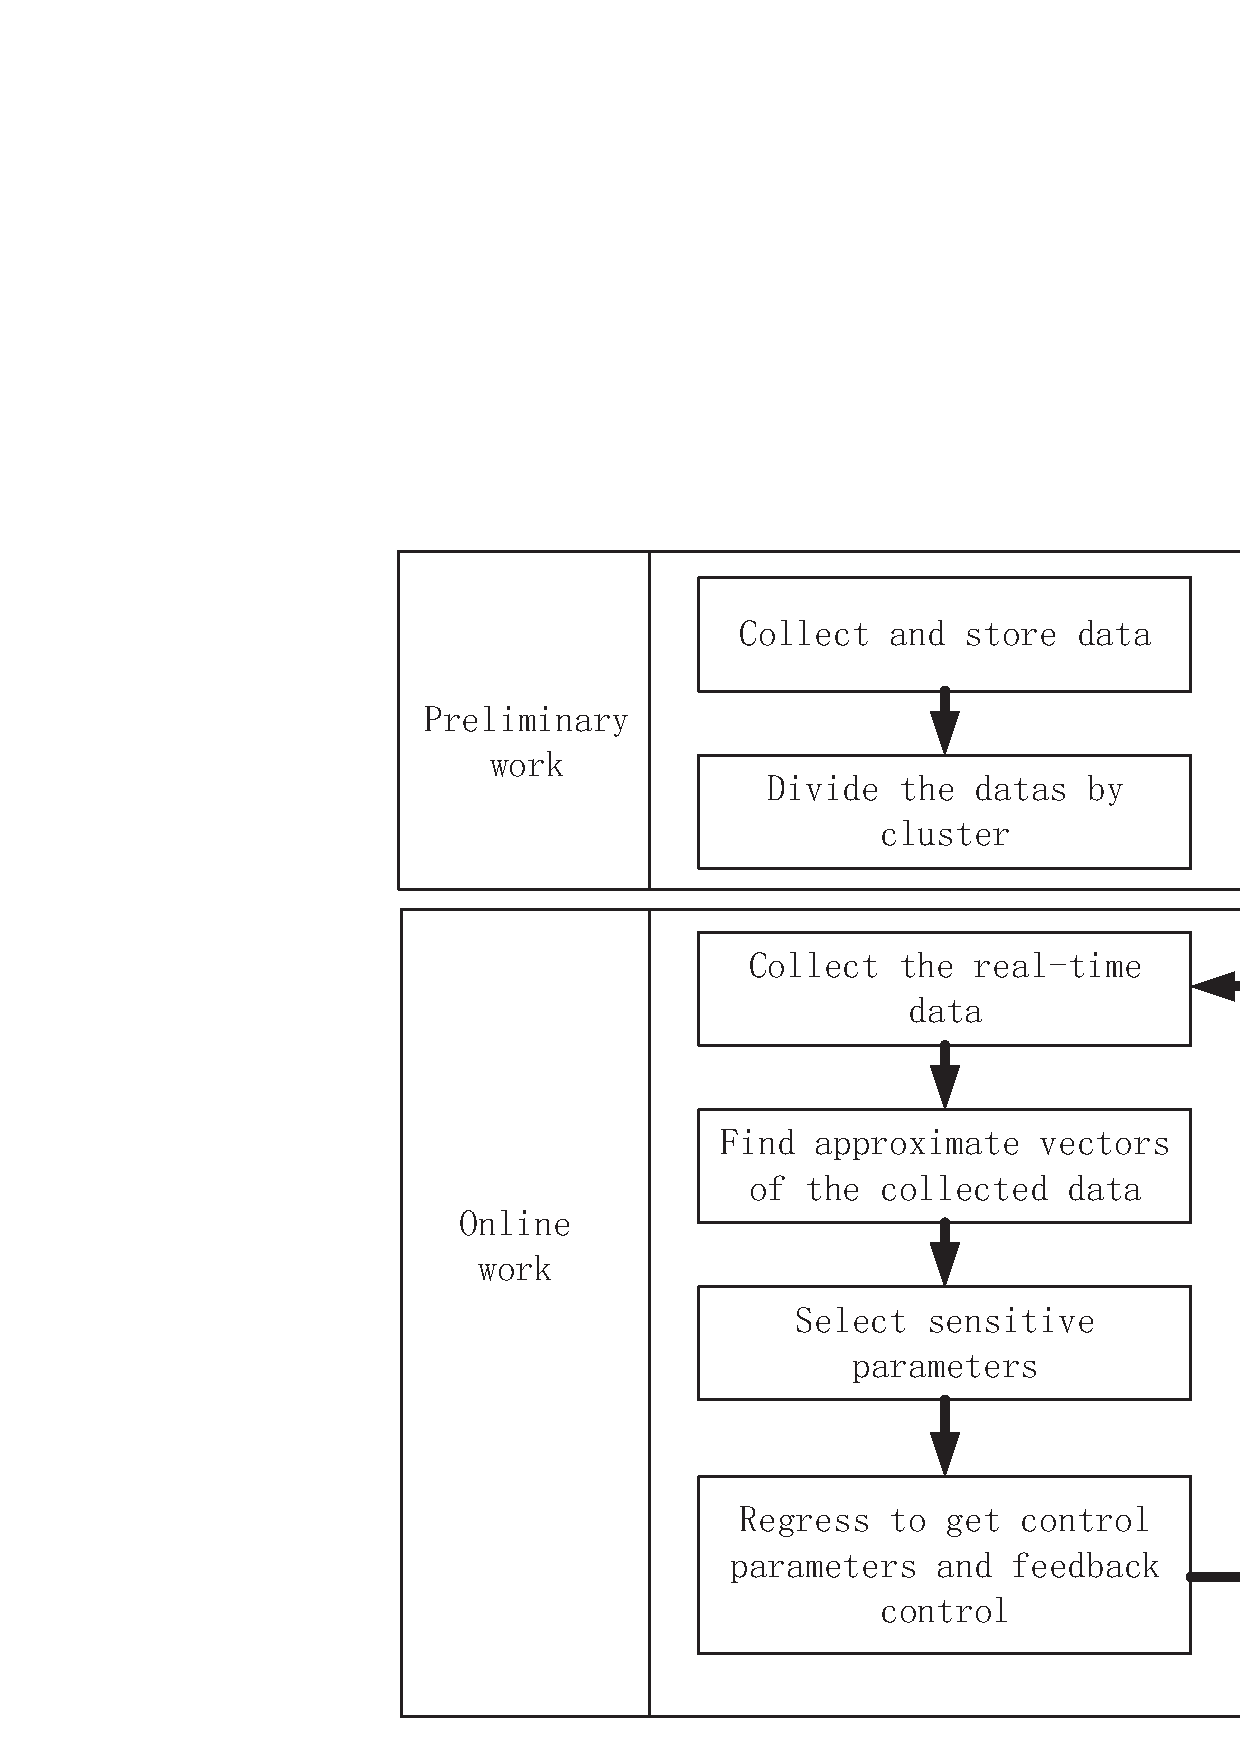
\includegraphics[width=.8\linewidth]{fig/mainwork/stepMap}
	\caption{The overall experimental flow chart}
	\figlabel{fig:stepMap}
\end{figure}

 In the preprocessing work, we let the robot climb the pipe with different diameters by using different parameters for thousands of times and we collect and store the data listed in the form like \figref{fig:data}.
\begin{figure}[H]
	\centering
	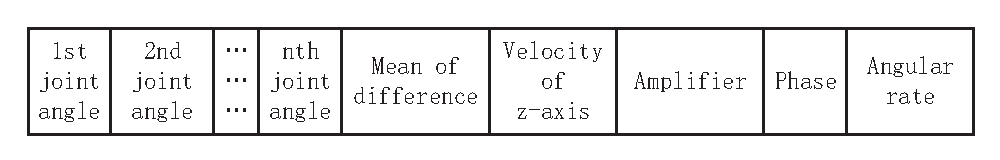
\includegraphics[width=\linewidth]{fig/mainwork/data}
	\caption{The structure of the data storage}
	\figlabel{fig:data}
\end{figure}

In this way, we define "Mean of difference" as $\frac{\sum_{i=1}^{n}(t^{(i)}-ma^{(i)})}{n} $ where n is the number of joints. $T=\begin{bmatrix}
t^{(1)} & t^{(2)} & \cdots & t^{(n)}
\end{bmatrix}$ is the desired joint angles and $MA=\begin{bmatrix}
ma^{(1)} & ma^{(2)} & \cdots & ma^{(n)}
\end{bmatrix}$ is the measured joint angles. The control vector is shown in Eq.\ref{controlV}
\begin{eqnarray}\label{controlV}
V_C=\begin{bmatrix}
A\\ 
\omega\\
\varepsilon
\end{bmatrix}
\end{eqnarray}

In Eq.\ref{controlV}, $A$ is the amplitude, $\omega$ is the phase, and the $\varepsilon$ is the angular rate. All of them come from Eq.\ref{basicRoll}.

We can get much collected data, which is the training data for snake-like robots. And then we cluster the training data in order to simplify the data processing.

After clustering, it reduces the time of data processing evidently. In robot's running time, we get the real-time data Periodically, we do the following steps. Firstly, we categorize the real-time data based on the clustering result in preprocessing. And then we select the most sensitive gait parameter according to the entropy variance. At last, we use the idea of regression to modify the sensitive gait parameter and keep the other gait parameters unchanged.

\subsection{Implementation of Clustering by $Kmeans++$}
In this research, collected data in preprocessing is a large-scale data set. As $kmeans++$ algorithm has high efficiency and scalability for a large-scale data set, we adopt $kmeans++$ for clustering. We classify training set into $N_{k}$ blocks. The clustering process is divided into the following steps:

\begin{itemize}
	\item Step 1: Randomly select a point in the training set as the first cluster center.
	\item Step 2: For the $k_{th}$ center, select the point which has the largest  distance to the $(k-1)$ centers in the current training set
	%prework step2
	\begin{eqnarray}\label{clu_step2}
	\left\{
	\begin{array}{lr}
	F_{c}\left ( P^{\left (  i\right )} \right ) = \sum_{j=1}^{k-1}\left \| X^{\left ( j-1 \right )}-P^{\left (  i\right )} \right \|_{2}\\
	k = $arg$\max \limits_{i}{(F_{C}(P^{(i)}))}
	\end{array}
	\right.
	\end{eqnarray}
	\begin{figure}[H]
		\centering
		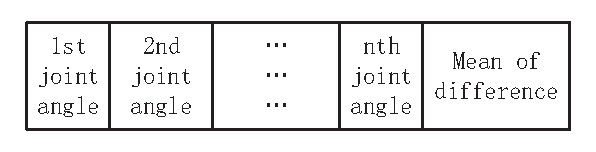
\includegraphics[height=0.5in]{fig/mainwork/data2}
		\caption{Data vector used in clustering and regression}
		\figlabel{fig:data2}
	\end{figure}
	$P^{(i)}$ is a data(\figref{fig:data2}) in the training set. $X^{(j)}$ is the $j_{th}$ cluster center. $S^{(P)}$ is the  training set. For the initial cluter center $X^{(k)}$, we have $X^{(k)}\in S^{(P)}$ and $X^{(k)}$ is the vector $P^{(i)}$ which corresponds to the result of Eq.\ref{clu_step2}. 
	\item Step 3: Repeat Step 1 and Step 2 until $N_{k}$ cluster centers have been confirmed.
	\item Step 4: After confirming $N_{k}$ cluster center, we categorize every vector in training set based on Eq.\ref{clu_step4}.
	%prework step4
	\begin{eqnarray}\label{clu_step4}
	C^{(i)} = arg\min \limits_{k}{(||P^{(i)}-X^{(k)}||_{2})}
	\end{eqnarray}
	In this equation, $C^{(i)}$ is the flag of category which the vector $P^{(i)}$ belongs to.
	\item Step 5: Refresh the cluster centers according to clustering result by the Eq.\ref{clu_step5}
	%prework step5
	\begin{eqnarray}\label{clu_step5}
	X^{(k)}=\frac{\sum_{i}\{C^{(i)}=k)\}P^{(i)}}{\sum_{i}\{C^{(i)}=k\}}
	\end{eqnarray}
	\item Step 6: iterate Step 4 and 5 until the cluster centers change in a small range.
\end{itemize}

After finishing the clustering, the result is stored in two parts:

\begin{itemize}
	\item The corresponding relationship between each vector in training set and the center of the cluster it belongs to.
	\item The data vectors of each cluster center.
\end{itemize}

With $Kmeans++$, the collected data can be divided into several clusters. In this way, we can do it the best to make the number of data in each cluster to be close.

\subsection{Parameter selection by entropy variance}

%classification
\subsubsection{Real-time data categorization}

Every time we get the real-time data, we relegate it to the certain cluster by Eq.\ref{cluster}.
\begin{eqnarray}\label{cluster}
C=arg\min \limits_{k}{(||X^{(k)}-P_{t}||_{2})} \, ,&X^{(C)}\in S^{(X)}
\end{eqnarray}

$S^{(X)}$ is the cluster center set. $X^{(C)}$ is the closet vector to the real-time vector $P_t$. And $X^{(k)}$ is the $i_{th}$ cluster center of the cluster center set $S^{(X)}$ . With $Euclidian \; Distance \; Formula$, we make a prediction on the similarity between two vectors.

\subsubsection{The selection of the preponderant data}

After categorization of real-time data, we select those preponderant vectors whose Z-axis velocity are bigger than current(Eq.\ref{preponderant}).
%find out preponderant
\begin{eqnarray}\label{preponderant}
S^{(V)}=\{P^{(i)}|V_{z}^{(i)}\geq V_{z}^{P_{t}} \; , \; P^{(i)}\in S^{(C)}\}
\end{eqnarray}

$S^{(C)}$ is all the vectors which belong to the cluster with the cluster center $X^{(C)}$. $V_{z}^{(i)}$ is the vertical velocity component of the vector $P^{(i)}$ and $V_{z}^{(P_{t})}$ is the vertical velocity component of the real-time data vector. $S^{(V)}$ is the set of all the preponderant vectors for regression.

\subsubsection{The selection of the sensitive parameter}

We adopt entropy variance as the reference to select the parameter which should be modified. The steps of selecting the sensitive parameter are as follows.

\begin{itemize}
	\item Step 1: We take the preprocessing operation to discrete the preponderant data (Eq.\ref{quantification}).
	%quantification
	\begin{eqnarray}\label{quantification}
	V_{new}^{(i)}=\left\{
	\begin{array}{lr}
	\left \lfloor \frac{V_{z}^{(i)}}{L_{D}} \right \rfloor&V_{z}^{(i)}> 0\\
	\\
	\left \lceil \frac{V_{z}^{(i)}-L_{D}}{L_{D}} \right \rceil&V_{z}^{(i)}\leq 0
	\end{array}
	\right.
	\end{eqnarray}
	
	In Eq.\ref{quantification}, $L_{D}$ is the adjustable step length for discretization. We eventually get the velocity discrete sequence:
	\begin{eqnarray}\label{newMember}
	V_{new}^{(Z)}=\begin{bmatrix}
	V_{new}^{(1)} & V_{new}^{(2)} & V_{new}^{(3)} & V_{new}^{(4)} & \cdots & \cdots
	\end{bmatrix}
	\end{eqnarray}
	
	\item Step 2: There are a variety of possible values for each gait parameter. Thus, in order to record all the possible values, we make a set $S_{ij}^{(P)}$ which is the data set of $j_{th}$ possible value of the gait parameter $i$. And value of $i$ is from 0 to 2 corresponding to amplitude, phase and angular rate respectively. We calculate the entropy about the vertical velocity of the $j_{th}$ possible value of the gait parameter $i$ by Eq.\ref{entropy} as well as the entropy variance of the gait parameter $i$ by Eq.\ref{var_entropy}. In Eq.\ref{entropy}, $p(v_{z})$ is the appearance rate of each member in the velocity discrete sequence as Eq.\ref{newMember}. In Eq.\ref{var_entropy}, $E_{ij}^{(H)}$ is the mean of velocity of  the $j_{th}$ possible value of the gait parameter $i$ and $N_{i}$ is the number of possible values of the gait parameter $i$.
	%entropy
	\begin{eqnarray}\label{entropy}
	H(S_{ij}^{(P)})=-\sum _{v_{z}\in V_{new}^{(Z)}}p(v_{z})log_{2}p(v_{z})
	\end{eqnarray}
	
	%entropy variance
	\begin{eqnarray}\label{var_entropy}
	Var_{i}^{(H)}=\frac{\sum _{N_{i}}(H(S_{ij}^{(P)})-E_{ij}^{(H)})^{2}}{N_{i}}
	\end{eqnarray}
	
	\item Step 3: We normalize the entropy variance (Eq.\ref{normalize}) and randomly select the sensitive gait parameters by roulette method (\figref{fig:Roulette}) to avoid the selection getting stuck in the high probability event.
	%normalize entropy variance
	\begin{eqnarray}\label{normalize}
	R_{i}^{(var)}=\frac{Var_{i}^{(H)}}{\sum Var^{(H)}}
	\end{eqnarray}
	
	\begin{figure}[H]
		\centering
		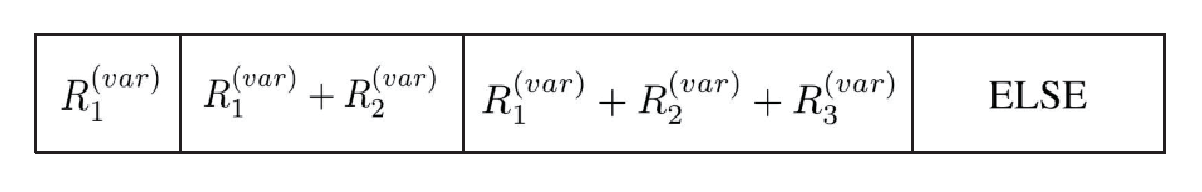
\includegraphics[width=\linewidth]{fig/mainwork/Roulette}
		\caption{Sensitive parameter selection by roulette method}
		\figlabel{fig:Roulette}
	\end{figure}
\end{itemize}

After the calculation of gait parameters' entropy variance. the sensitive parameter will be found. And then the selected parameter is used in the regression control later.


\subsection{Assignment of the sensitive parameter by weighted regression}

In this research, we take weighted regression to get the value of the sensitive gait parameter and use the gradient descent method to solve the weighted least squares problem in fitting regression function.

\begin{itemize}
	\item Step 1: List the fitting prediction function(Eq.\ref{fitfunction})
	%fitting and estimation function
	\begin{eqnarray}\label{fitfunction}
	F_{w}(P_{t})=W^{T}P_{t}\,,&W=\begin{bmatrix}w_{1}\\ w_{2}\\ \vdots \\ w_{m}\end{bmatrix}
	\end{eqnarray}
	
	In Eq.\ref{fitfunction}, $W$ is the coefficient sequence of the fitting equation and $m$ is the number of coefficients where $P_{t}$ is the collected vector in real-time with the model of  \figref{fig:data2}. Then we can get the error function(Eq.\ref{estimate}) which takes the square of error as the estimation with $n$ being the number of data of $S^{(V)}$ and $Q$ being the vector consisting of the sensitive parameter component of the vector $P^{(i)}( P^{(i)} \in P)$.
	%Square sum as an estimation
	\begin{eqnarray}\label{estimate}
		D(W)=\frac{1}{2n}(F_{w}(P)^{T}-Q)^{T}(F_{w}(P)^{T}-Q)
	\end{eqnarray}
	\begin{eqnarray}
		P=\begin{bmatrix}P^{(1)}&P^{(2)}  &\cdots  &P^{(n)} \end{bmatrix}, &P^{(i)}\in S^{(V)}
	\end{eqnarray}
	\begin{eqnarray}
		Q=\begin{bmatrix}Q^{(1)}& Q^{(2)}& \cdots & Q^{(n)}\end{bmatrix}^{T}
	\end{eqnarray}
	
	To get the best-fit coefficient sequence $W$ by the minimum $D(w)$, according to gradient descent method, we turn the Eq.\ref{estimate} into Eq.\ref{Gradde}.
	%Gradient descent
	\begin{eqnarray}\label{Gradde}
	\nabla_{w}D=\frac{1}{n}P(F_{w}(P)^{T}-Q)
	\end{eqnarray}
	
	\item Step 2: Perform the weighted operation on preponderant data vector to ensure the estimate result of fitting is good (Eq.\ref{WeiGradde}).
	%weighted gradient
	\begin{eqnarray}
	\nabla_{w}D=\frac{1}{n}PM(F_{w}(P)^{T}-Q)
	\end{eqnarray}
	\begin{eqnarray}\label{WeiGradde}
	M=\begin{bmatrix}
	\frac{V_{z}^{(1)}}{L_{s}}&0&\cdots&0\\
	0&\frac{V_{z}^{(2)}}{L_{s}}&\ddots&0\\
	\vdots&\ddots&\ddots&0\\
	0&\cdots&0&\frac{V_{z}^{(n)}}{L_{s}}
	\end{bmatrix}
	\end{eqnarray}
	In Eq.\ref{WeiGradde}, $L_s$ is the learning step and $M$ is the learning rate matrix.
	
	\item Step 3: Fit the coefficient vector by Eq.\ref{fit}.
	%fitting the parameters
	\begin{eqnarray}\label{fit}
	W=W-\nabla_{w}D
	\end{eqnarray}
	
	In this way, the coefficient sequence $W$ is updated. And then we assign the predicting result to the sensitive parameter(Eq.\ref{result}).
	%compensation result
	\begin{eqnarray}\label{result}
	Q=F_{w}(P_{t})=W^{T}P_{t}
	\end{eqnarray}
	After this the new predicting result is produced.
	
	\item Step 4: Iterate the steps above until we acquire the best-fit coefficient. The value of $W$ is stable finally.
\end{itemize}

When the iteration is stopped, the best-fit coefficient $W_{best}$ will be got. By applying $W_{best}$ to Eq.\ref{result}, we can get the regression value of the sensitive parameter. This value will be used in the robot control. It is worth noting that we only modify the sensitive parameter and others remain the same value.
\section{SIMULATION}
We use the rolling gait as the basic gait for the simulation. To verify the adaptive control of the robots in their motion, we simulate the robots' climbing on pipes with different diameters under the robot simulation platform VREP.

The simulation process can be divided into two categories: training and motion simulation. And we divide motion simulation into two parts: the adaptable motion along variable diameter pipes and the adaptable motion along straight pipes with different diameter .

\subsection{Training process}

In the data acquisition process, we make the robot climb along the 25cm and 35cm pipes for thousands of times respectively under different parameters. The interval of amplitude $A$, phase $\varepsilon$ and angular rate $\omega$ are $[40, \, 80]$, $[0, \, 5]$ and $[1.5, \, 3]$ respectively. What's more, the step of $A$ is 5, the step of $\varepsilon$ is 1 and the step of $\omega$ is 0.5. The state of the robot will change during the course of the movement. We make the robot climb with different combination of parameters and collect the data. Then we can eventually collect more than 20 thousand volumes of training data. In the preprocessing process, we cluster the training data. We set the number of clusters as 25 or so to ensure the uniform distribution of clustering. The number of data for each class is $1000 \pm 500 $ (\figref{fig:clustersize}).

\begin{figure}[t]
	\centering
	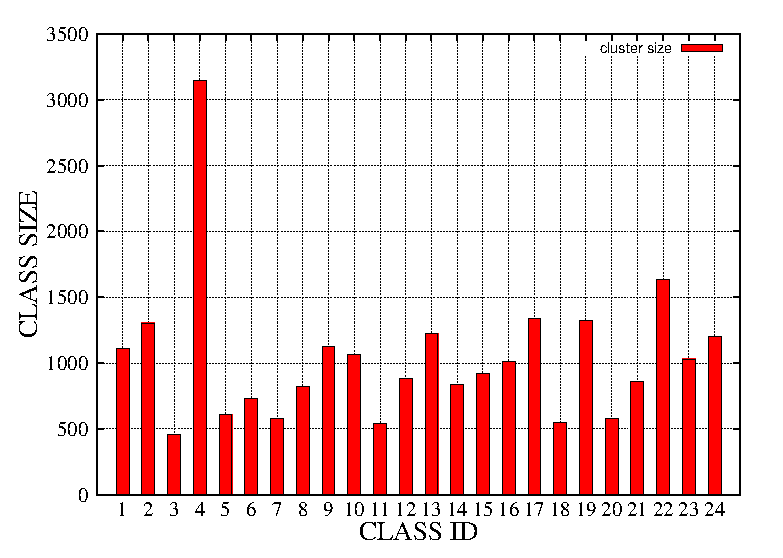
\includegraphics[width=0.6\linewidth]{fig/experiment/170912/cluster}
	\caption{The result of clustering about member size of each class}
	\figlabel{fig:clustersize}
\end{figure}

\subsection{the adaptable motion along variable diameter pipes}

The simulation in this part is 35cm to 25cm vertical pipe climbing simulation (\figref{fig:ccurve1}) and 25cm to 35cm vertical pipe climbing simulation (\figref{fig:ccurve2}). From the two simulation results we can find that the robot can adaptively learn to find better motion control parameters than current. Next, the two groups of simulation will be analyzed in detail.

\subsubsection{For 35cm to 25cm pipe climbing simulation}

The results are shown in \figref{fig:ccurve1}. In 0s to 15s, the robot changes itself from the stretch state to compressed state. Since the robot does not get the diameter of pipe, it spends a long time in adapting to the unknown pipe. So in this phase, its velocity is close to zero. In 15s to 40s, the robot climb along the pipe with 35cm diameter. In this phase, amplitude $A$, phase $\varepsilon$ and angular rate $\omega$ are all increasing and all of the them will be stable finally. About 50s, the robot reach the interface where the diameter changes. As the pipe changes obvious, the robot can not grasp the 25cm pipe immediately, which causes the velocity of the robot fluctuate around zero. The robot keeps learning and autonomously adjust its parameters to continue its climbing motion. From the \figref{fig:bsa} and \figref{fig:bsp}, it can be found that the amplitude and phase are increasing in this phase, which make the robot continue moving up.

Eventually all control parameters as well as velocity are stable. It shows that under this control strategy, the robot can adjust its parameters autonomously to adapt to the environment.

\begin{figure}[!t]
	\centering
	\subfigure[t= 0.0s]{
		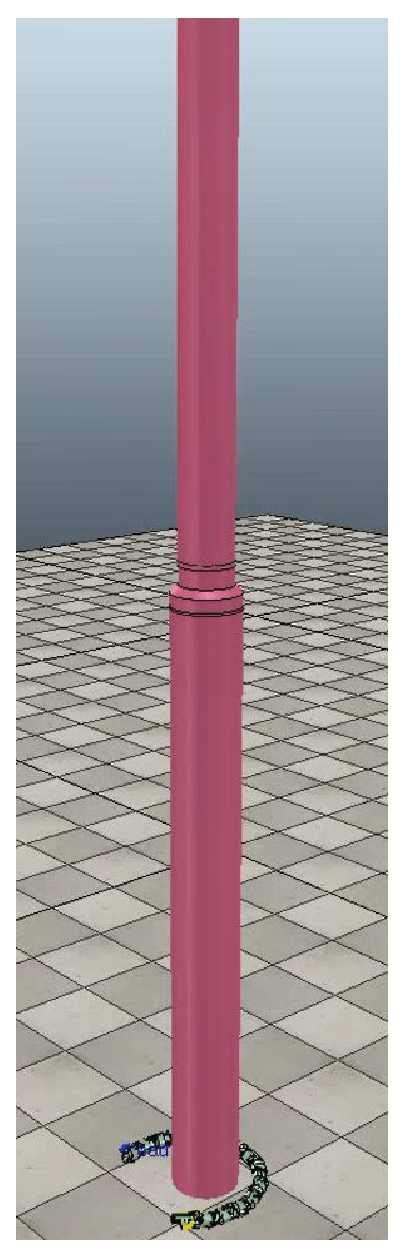
\includegraphics[height=2in,width=.12\textwidth]{fig/experiment/170912/bs0}
	}
	\subfigure[t=20.2s]{
		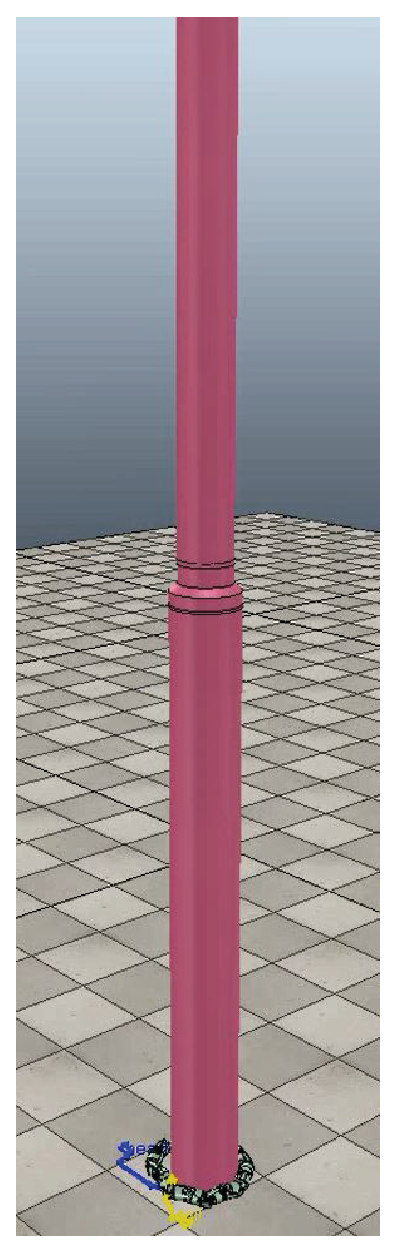
\includegraphics[height=2in,width=.12\textwidth]{fig/experiment/170912/bs1}
	}
	\subfigure[t=39.8s]{
		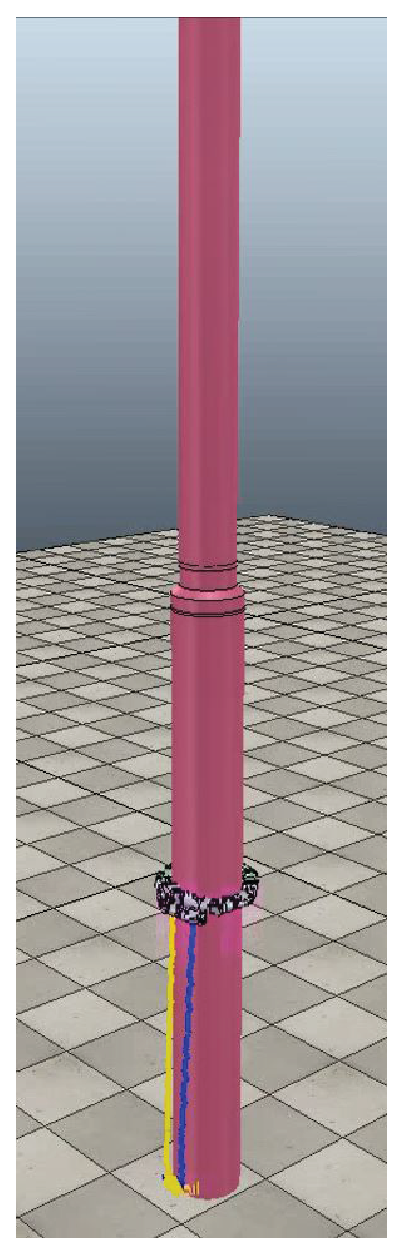
\includegraphics[height=2in,width=.12\textwidth]{fig/experiment/170912/bs2}
	}
	
	
	\subfigure[t=50.5s]{
		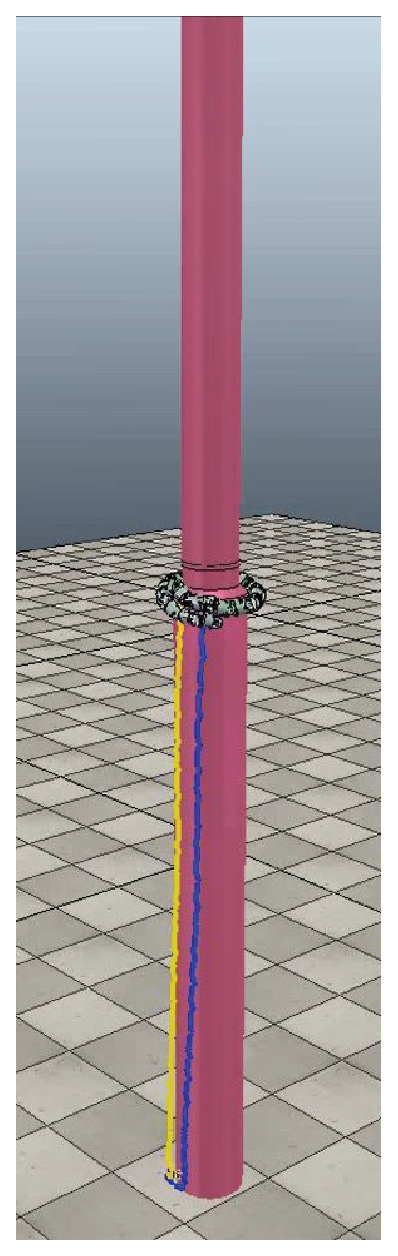
\includegraphics[height=2in,width=.12\textwidth]{fig/experiment/170912/bs3}
	}
	\subfigure[t=60.0s]{
		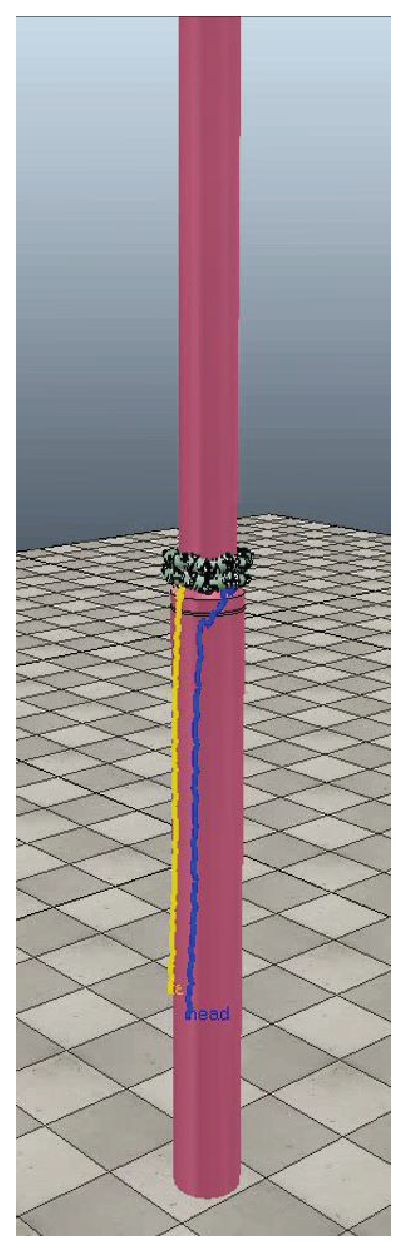
\includegraphics[height=2in,width=.12\textwidth]{fig/experiment/170912/bs4}
	}
	\subfigure[t=64.5s]{
		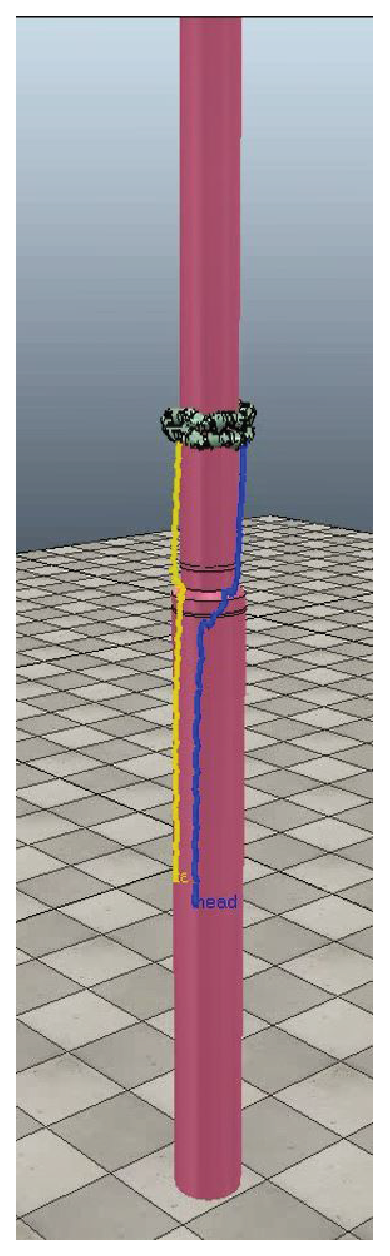
\includegraphics[height=2in,width=.12\textwidth]{fig/experiment/170912/bs5}
	}
	
	\subfigure[Amplifier versus Time]{
		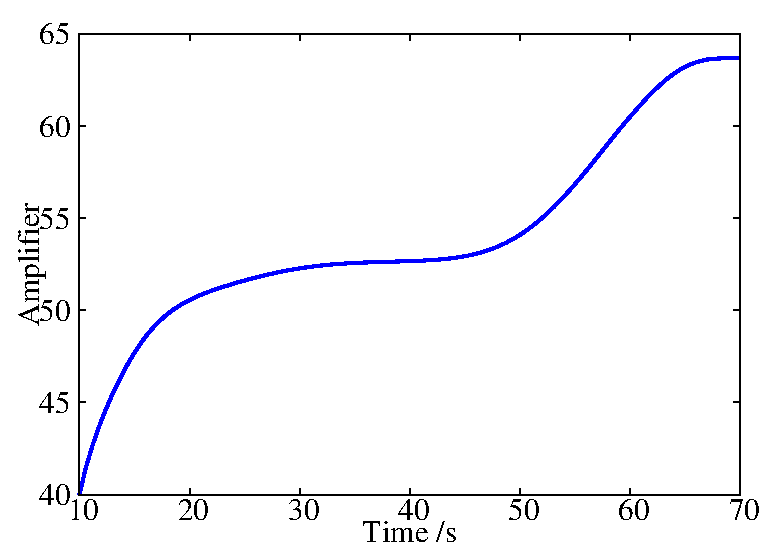
\includegraphics[width=.2\textwidth]{fig/experiment/170912/bsamplifier}
		\figlabel{fig:bsa}
	}
	\subfigure[Phase versus Time]{
		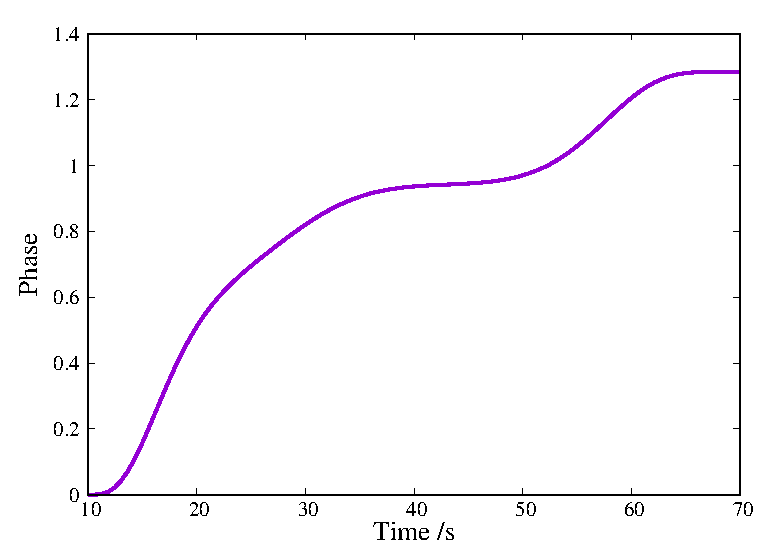
\includegraphics[width=.2\textwidth]{fig/experiment/170912/bsphase}
		\figlabel{fig:bsp}
	}
	
	\subfigure[Angular rate versus Time]{
		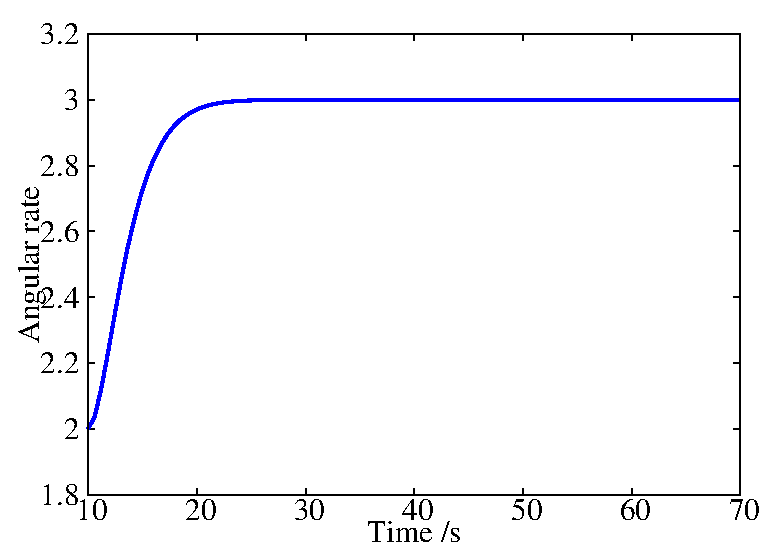
\includegraphics[width=.2\textwidth]{fig/experiment/170912/bsangrate}
		\figlabel{fig:bsw}
	}
	\subfigure[velocity versus Time]{
		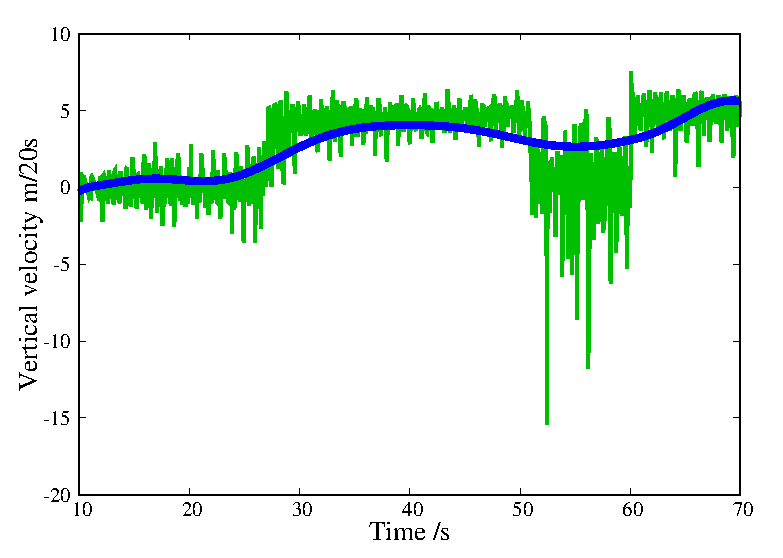
\includegraphics[width=.2\textwidth]{fig/experiment/170912/bsv}
		\figlabel{fig:bsv}
	}
	\caption{The movement process and the curves of parameters changing in the motion along the 35cm to 25cm pipe}
	\figlabel{fig:ccurve1}
\end{figure}

\begin{figure}[!t]
	\centering
	\subfigure[t= 0.0s]{
		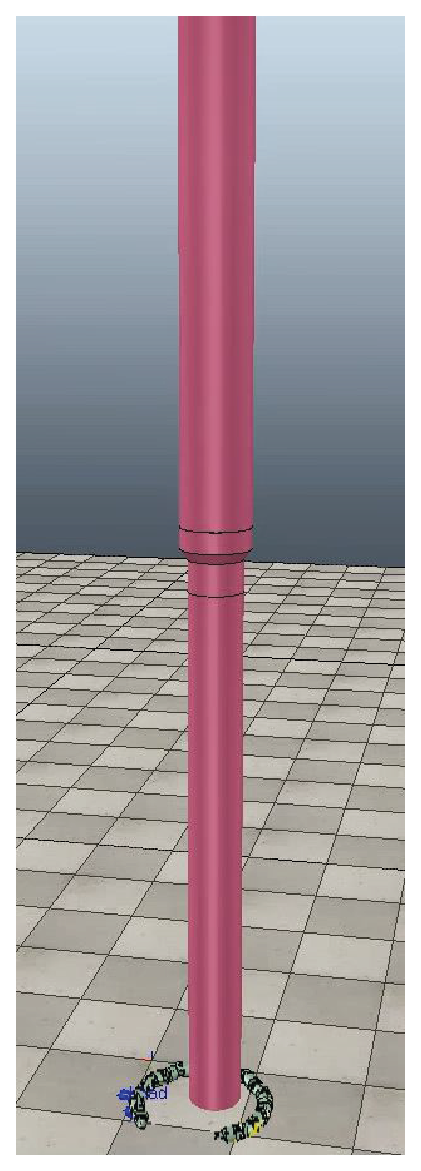
\includegraphics[height=2in,width=.12\textwidth]{fig/experiment/170912/sb0}
	}
	\subfigure[t=29.2s]{
		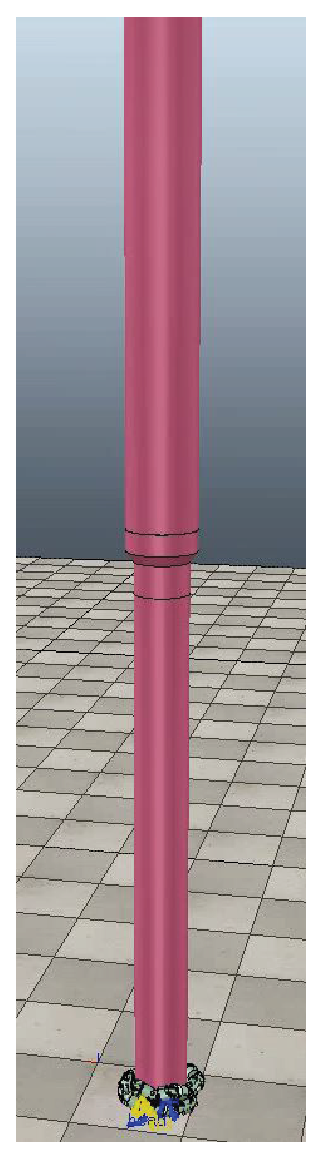
\includegraphics[height=2in,width=.12\textwidth]{fig/experiment/170912/sb1}
	}
	\subfigure[t=40.5s]{
		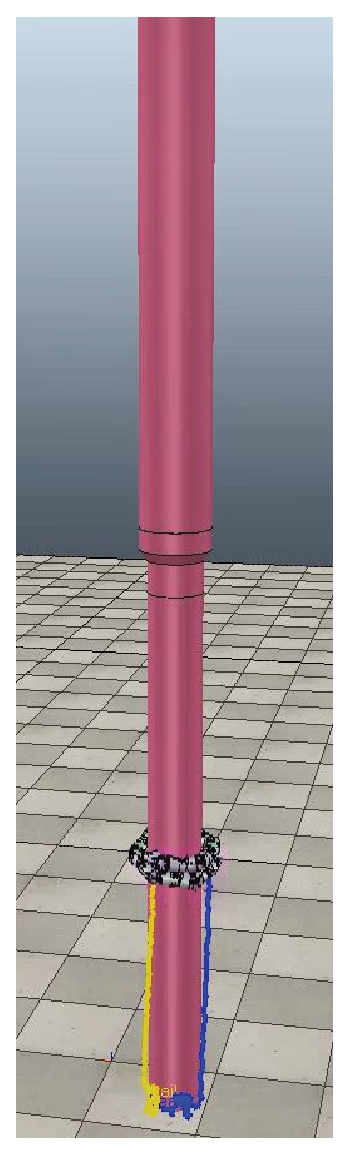
\includegraphics[height=2in,width=.12\textwidth]{fig/experiment/170912/sb2}
	}
	
	\subfigure[t=55.0s]{
		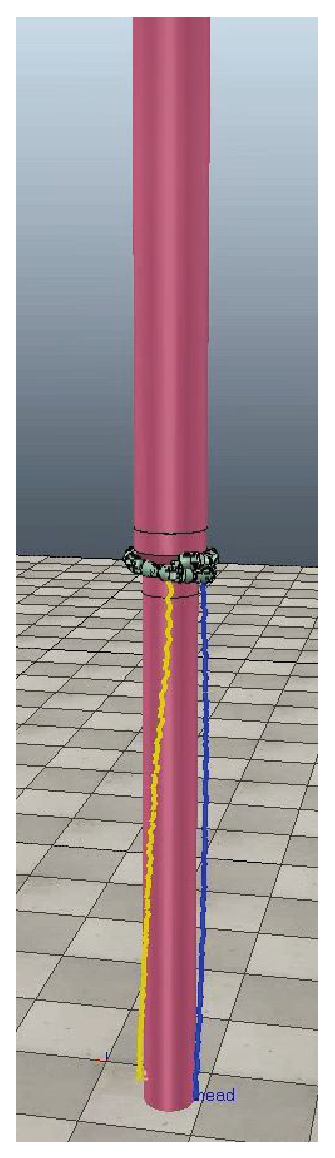
\includegraphics[height=2in,width=.12\textwidth]{fig/experiment/170912/sb3}
	}
	\subfigure[t=58.9s]{
		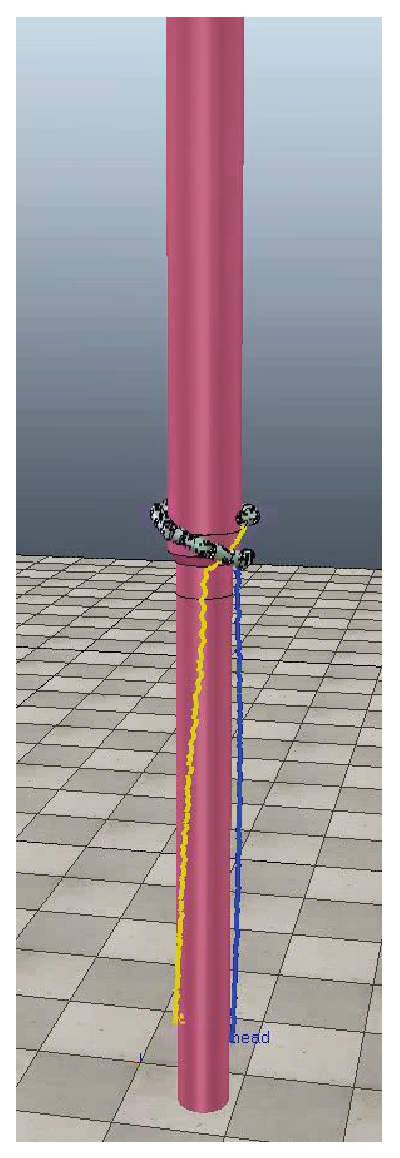
\includegraphics[height=2in,width=.12\textwidth]{fig/experiment/170912/sb4}
	}
	\subfigure[t=66.0s]{
		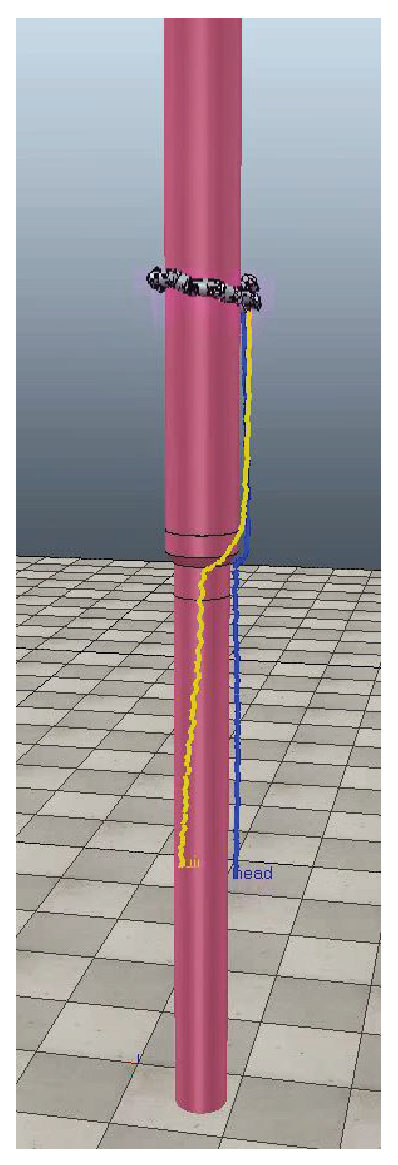
\includegraphics[height=2in,width=.12\textwidth]{fig/experiment/170912/sb5}
	}
	\subfigure[Amplifier versus Time]{
		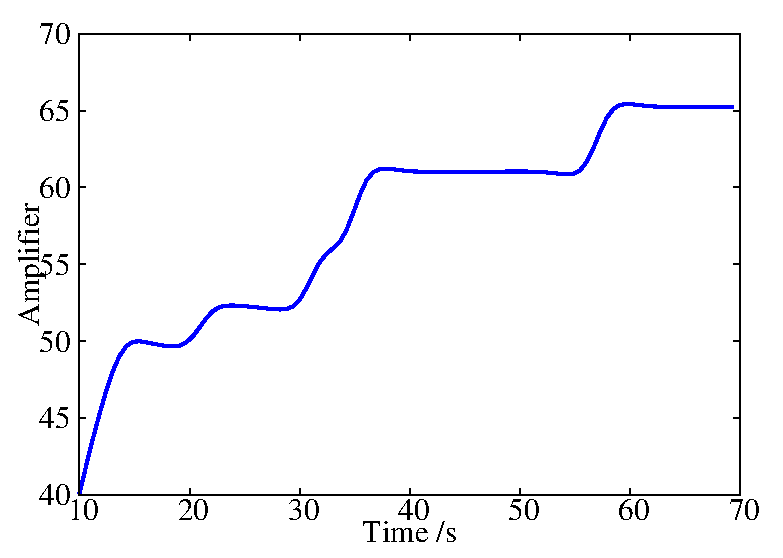
\includegraphics[width=.2\textwidth]{fig/experiment/170912/sbamplifier1}
		\figlabel{fig:sba}
	}
	\subfigure[Phase versus Time]{
		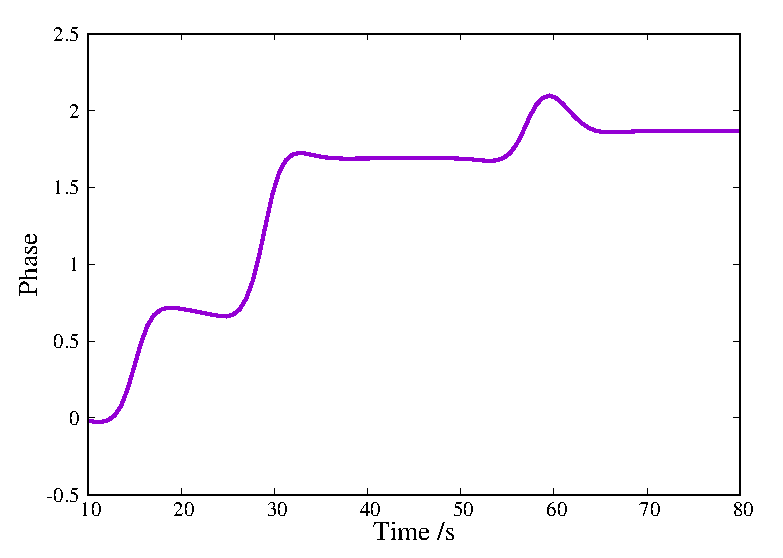
\includegraphics[width=.2\textwidth]{fig/experiment/170912/sbphase}
		\figlabel{fig:sbp}
	}
	
	\subfigure[Angular rate versus Time]{
		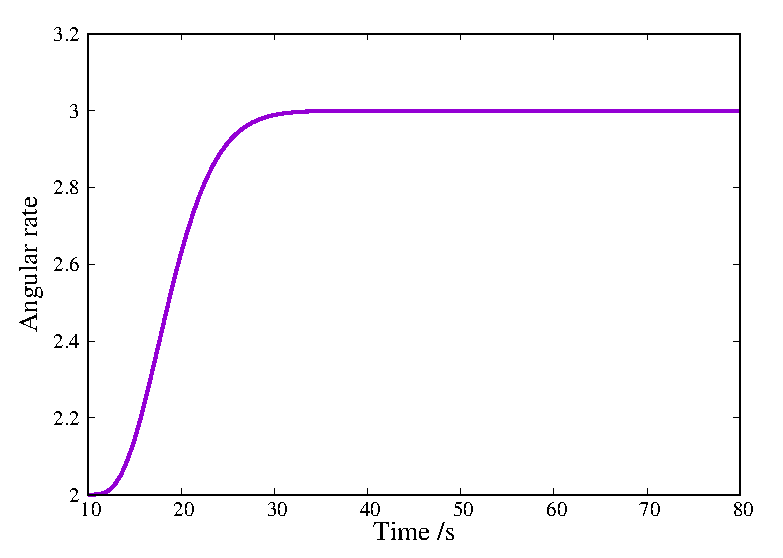
\includegraphics[width=.2\textwidth]{fig/experiment/170912/sbangrate}
		\figlabel{fig:sbw}
	}
	\subfigure[velocity versus Time]{
		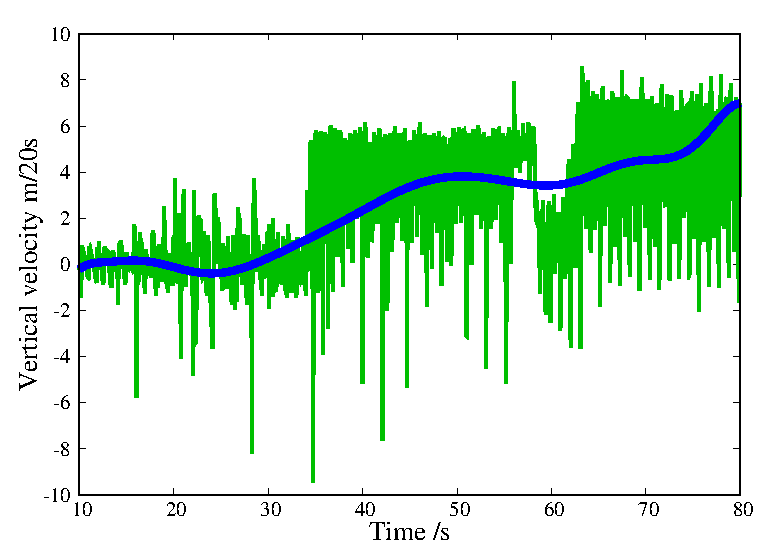
\includegraphics[width=.2\textwidth]{fig/experiment/170912/sbv}
		\figlabel{fig:sbv}
	}
	\caption{The movement process and the curves of parameters changing in the motion along the 25cm to 35cm pipe}
	\figlabel{fig:ccurve2}
\end{figure}

\subsubsection{For 25cm to 35cm pipe climbing simulation}
It is similar with the previous simulation, but the movement is different in the interface where the diameter changes. The results are shown in \figref{fig:ccurve2}. Firstly, the snake-like robot spend a lot of time to coil the 25cm pipeline. And then the robot adjust itself and finally its parameters reach stable. About 52s, the robot encounters the interface where the diameter changes. At this time the robot autonomously reduce amplitude slightly (\figref{fig:sba}) and then significantly increase  phase (\figref{fig:sbp}). In this way, the control strategy make the robot move itself from the 25cm part up to the 35cm part. When on the 35cm part, the robot will automatically increase the amplitude and decrease the phase shift until reaching the steady state.

Both simulations show that our method is effective to adapt the robot to climb along the variable diameter pipe.

\subsection{Contrast experiments on other straight pipes}

As the unknown environment in the real world is complex and volatile, there may be a movement environment different to the training environment. Our training environment is vertical pipes with 25cm or 35cm diameter. To ensure that this control strategy can be applied in many situation, we conduct several  independent simulations on 20cm, 25cm, 30cm, 35cm or 40cm straight pipe. The result of these simulations are shown in \figref{fig:scurve}. The simulations show that the robot can use our control strategy to catch the unknown pipe and adjust itself to a suitable climbing state. Next is the detailed analysis.

By observing the parameter curve we can find that the smaller diameter of the pipe is, the much more time the parameters need to spend in adjusting. All parameters finally reach a stable value and satisfy the requirements of movement. For the 40cm diameter pipe, the robot is not long enough to form a single ring to wrap the pipe (\figref{fig:D40}), in this case the influence made by phase $\varepsilon$ is very weak (\figref{fig:sphase}). For the 20cm diameter pipe, it is difficult for the robot to climb along the pipe only by increasing the amplitude $A$, because when the amplitude is too large, it will cause the snake-like robot curling up to a high degree, which is not conducive to climb. Therefore, to make the robot climb small diameter pipe, we need to constantly adjust the phase $\varepsilon$ to meet the amplitude $A$'s corresponding requirements. By observing the variation curve of the control parameters of the small diameter pipe, we can found that the phase $\varepsilon$ and the amplitude $A$ of the robot are coordinated in the process of self-regulation ( \figref{fig:samplifier})(\figref{fig:sphase}).

\begin{figure}[!t]
	\centering
	\subfigure[d=20cm]{
		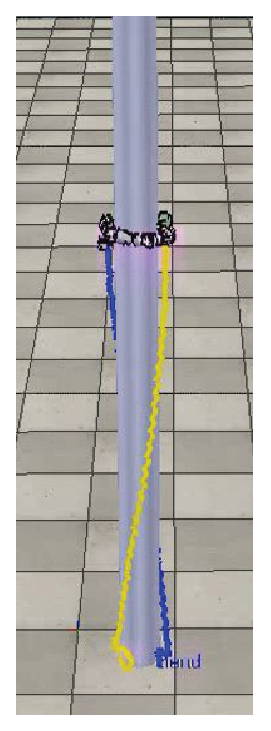
\includegraphics[height=2in,width=.12\textwidth]{fig/experiment/170912/D20}
		\figlabel{fig:D20}
	}
	\subfigure[d=25cm]{
		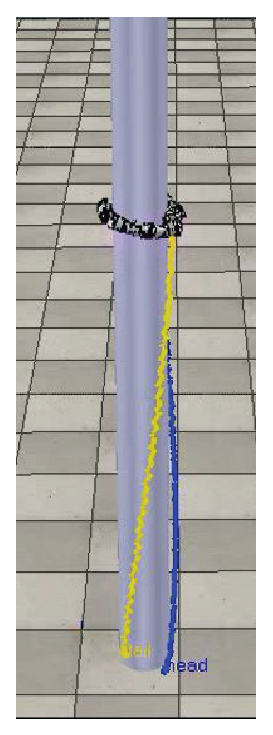
\includegraphics[height=2in,width=.12\textwidth]{fig/experiment/170912/D25}
		\figlabel{fig:D25}	
	}
	
	\subfigure[d=30cm]{
		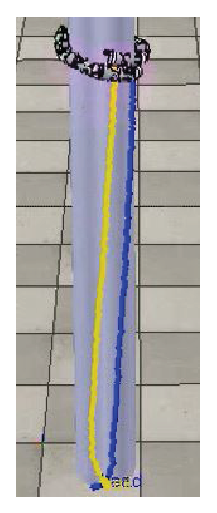
\includegraphics[height=2in,width=.12\textwidth]{fig/experiment/170912/D30}
		\figlabel{fig:D30}
	}
	\subfigure[d=35cm]{
		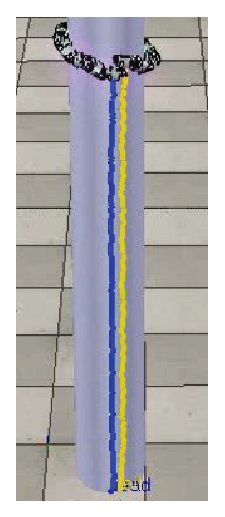
\includegraphics[height=2in,width=.12\textwidth]{fig/experiment/170912/D35}
		\figlabel{fig:D35}
	}
	\subfigure[d=40cm]{
		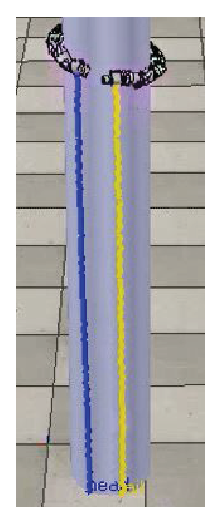
\includegraphics[height=2in,width=.12\textwidth]{fig/experiment/170912/D40}
		\figlabel{fig:D40}
	}
	
	\subfigure[Amplifier versus Time]{
		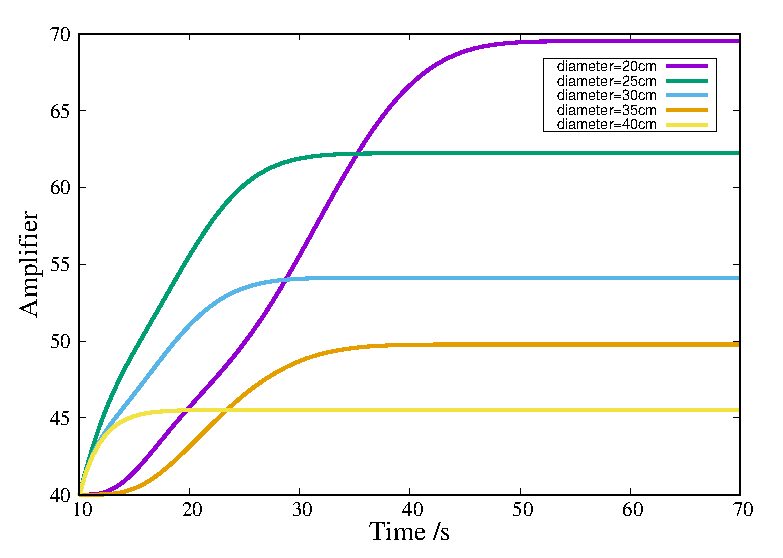
\includegraphics[width=.2\textwidth]{fig/experiment/170912/samplifier}
		\figlabel{fig:samplifier}
	}
	\subfigure[Phase versus Time]{
		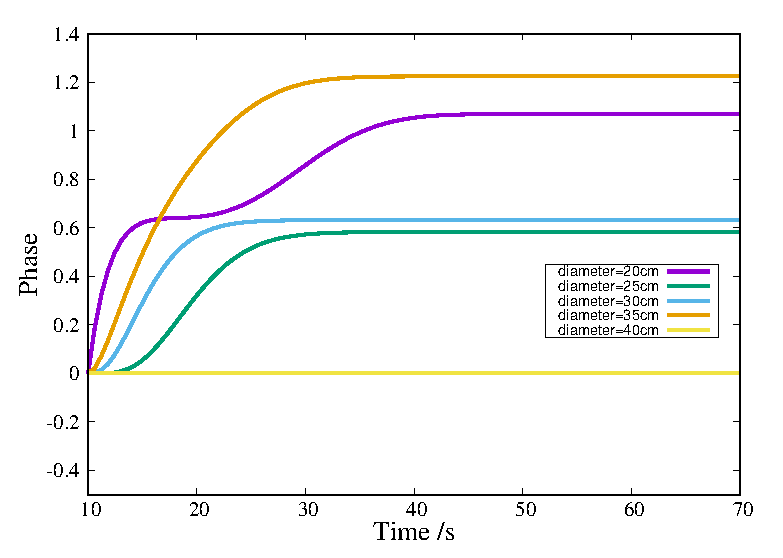
\includegraphics[width=.2\textwidth]{fig/experiment/170912/sphase}
		\figlabel{fig:sphase}
	}
	\subfigure[Angular rate versus Time]{
		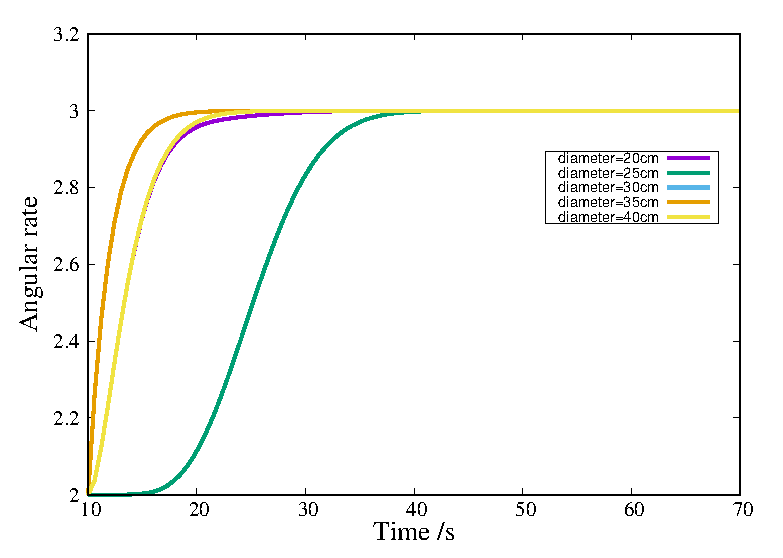
\includegraphics[width=.2\textwidth]{fig/experiment/170912/sarate}
		\figlabel{fig:sarate}
	}
	\subfigure[velocity versus Time]{
		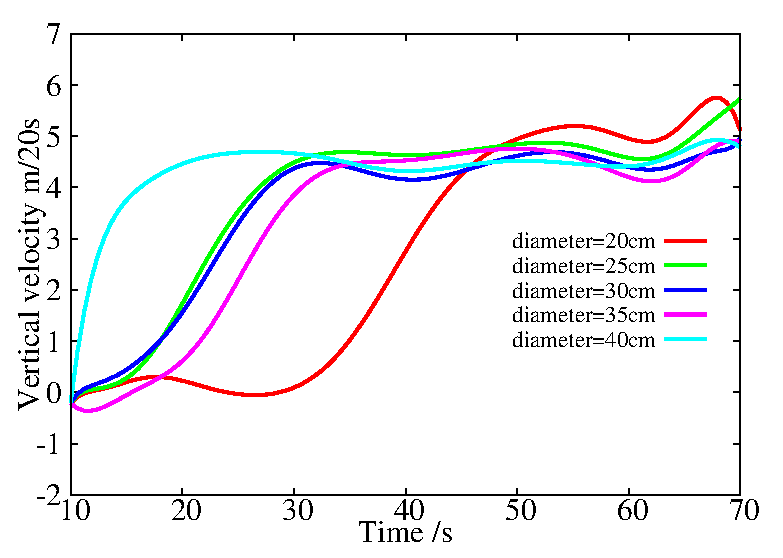
\includegraphics[width=.2\textwidth]{fig/experiment/170912/svel}
		\figlabel{fig:svelocity}
	}
	\caption{The comparison curve about parameters changing versus time in different diameter pipe climbing}
	\figlabel{fig:scurve}
\end{figure}

It is worth noting that, for all test environments, the movement velocity of the robot  ultimately fluctuate within a constant range  (\figref{fig:svelocity}). The diameter of the pipe only affects the velocity convergence rate. And also the control parameters of the robot will eventually become stable (\figref{fig:scurve}). This shows that the influence of the external environment to this control strategy is very weak. What's more, for the pipes that can be climbed, it will find the optimal control parameter.

The above simulations show that our control strategy can be applied to a lot of environment and is effective, too.

In conclusion, the simulations demonstrate that the adaptive control in robot's motion can be realized through our proposed framework in \figref{fig:stepMap}.

\section{Conclusion and future work}
This paper presents a framework for robot-based adaptive control based on reinforcement learning. We take Z-axis velocity as reinforcement signal and adopt regression to correct the robots' action. We simplify the runtime learning through clustering and transform the multiple regression into unit regression. Experiments show that the scheme is effective.

It is noteworthy that this method can be used not only in the case like climbing pipe in this experiment, but also in other robotic applications. We believe that the algorithm can adapt to the other corresponding scene, such as the unmanned vehicle's variable motion, the rugged ground motion of the serpentine robot and the simulated PID control as long as enough training data and clear moving purpose are given.

In the future work, we will improve the algorithm in the following ways. The hierarchical clustering\cite{HierarchicalKmeans}\cite{HierarchicalClusterBased} will be applied to the model to achieve uniform clustering to ensure that the data volume of each regression is consistent. Existing regression models will also be improved. What's more, we will carry out testing in much more complex climbing scene such as simulating trees in nature and bifurcate pipelines. We will develop much more complex rules for learning and running in much more complex environments.


% trigger a \newpage just before the given reference
% number - used to balance the columns on the last page
% adjust value as needed - may need to be readjusted if
% the document is modified later
%\IEEEtriggeratref{8}
% The "triggered" command can be changed if desired:
%\IEEEtriggercmd{\enlargethispage{-5in}}

% references section

% can use a bibliography generated by BibTeX as a .bbl file
% BibTeX documentation can be easily obtained at:
% http://mirror.ctan.org/biblio/bibtex/contrib/doc/
% The IEEEtran BibTeX style support page is at:
% http://www.michaelshell.org/tex/ieeetran/bibtex/
\bibliographystyle{IEEEtran}
% argument is your BibTeX string definitions and bibliography database(s)
\bibliography{ref}
%
% <OR> manually copy in the resultant .bbl file
% set second argument of \begin to the number of references
% (used to reserve space for the reference number labels box)

% that's all folks
\end{document}


